\documentclass[tikz,border=10pt]{standalone}
\usepackage{xcolor}
\usepackage{amsmath}
\usetikzlibrary{arrows.meta,calc,positioning}

\pagecolor{white}

\definecolor{fineblue}{RGB}{47,104,160}
\definecolor{workorange}{RGB}{218,132,40}
\definecolor{readgreen}{RGB}{42,142,92}
\definecolor{writered}{RGB}{190,72,82}
\definecolor{ink}{RGB}{42,48,56}
\definecolor{softgray}{RGB}{244,247,250}

\tikzset{
  flow/.style={-Latex, line width=1.05pt, draw=ink},
  residual/.style={-Latex, line width=1.15pt, draw=fineblue},
  readflow/.style={-Latex, line width=1.10pt, draw=readgreen},
  writeflow/.style={-Latex, line width=1.10pt, draw=writered},
  lab/.style={font=\small, align=center},
  tiny/.style={font=\scriptsize, align=center},
}

% Oblique grid plane using a fixed projection basis.
% #1 prefix, #2 origin, #3 columns, #4 rows, #5 color, #6 fill opacity
\newcommand{\gridplane}[6]{
  \begin{scope}[shift={#2}, x={(0.34cm,0.13cm)}, y={(0.54cm,-0.18cm)}]
    \coordinate (#1-o) at (0,0);
    \coordinate (#1-a) at (#3,0);
    \coordinate (#1-b) at (0,#4);
    \coordinate (#1-c) at (#3,#4);
    \fill[#5!8, opacity=#6] (#1-o) -- (#1-a) -- (#1-c) -- (#1-b) -- cycle;
    \foreach \i in {0,...,#3} {
      \draw[#5!35, line width=0.25pt] (\i,0) -- (\i,#4);
    }
    \foreach \j in {0,...,#4} {
      \draw[#5!35, line width=0.25pt] (0,\j) -- (#3,\j);
    }
    \draw[#5, line width=0.85pt] (0,0) -- (#3,0) -- (#3,#4) -- (0,#4) -- cycle;
  \end{scope}
}

% Draw extra fine grid lines without changing the logical cell coordinates.
% #1 origin, #2 columns, #3 rows, #4 subdivision factor, #5 color
\newcommand{\subgrid}[5]{
  \begin{scope}[shift={#1}, x={(0.34cm,0.13cm)}, y={(0.54cm,-0.18cm)}]
    \pgfmathtruncatemacro{\imax}{#2*#4}
    \pgfmathtruncatemacro{\jmax}{#3*#4}
    \foreach \i in {0,...,\imax} {
      \draw[#5!18, line width=0.16pt] ({\i/#4},0) -- ({\i/#4},#3);
    }
    \foreach \j in {0,...,\jmax} {
      \draw[#5!18, line width=0.16pt] (0,{\j/#4}) -- (#2,{\j/#4});
    }
  \end{scope}
}

% Highlight a cell region on one oblique plane.
% #1 prefix, #2 origin, #3 i, #4 j, #5 w, #6 h, #7 color, #8 opacity
\newcommand{\cellpatch}[8]{
  \begin{scope}[shift={#2}, x={(0.34cm,0.13cm)}, y={(0.54cm,-0.18cm)}]
    \coordinate (#1-p0) at (#3,#4);
    \coordinate (#1-p1) at (#3+#5,#4);
    \coordinate (#1-p2) at (#3+#5,#4+#6);
    \coordinate (#1-p3) at (#3,#4+#6);
    \fill[#7!30, opacity=#8] (#1-p0) -- (#1-p1) -- (#1-p2) -- (#1-p3) -- cycle;
    \draw[#7, line width=1.0pt] (#1-p0) -- (#1-p1) -- (#1-p2) -- (#1-p3) -- cycle;
  \end{scope}
}

\begin{document}
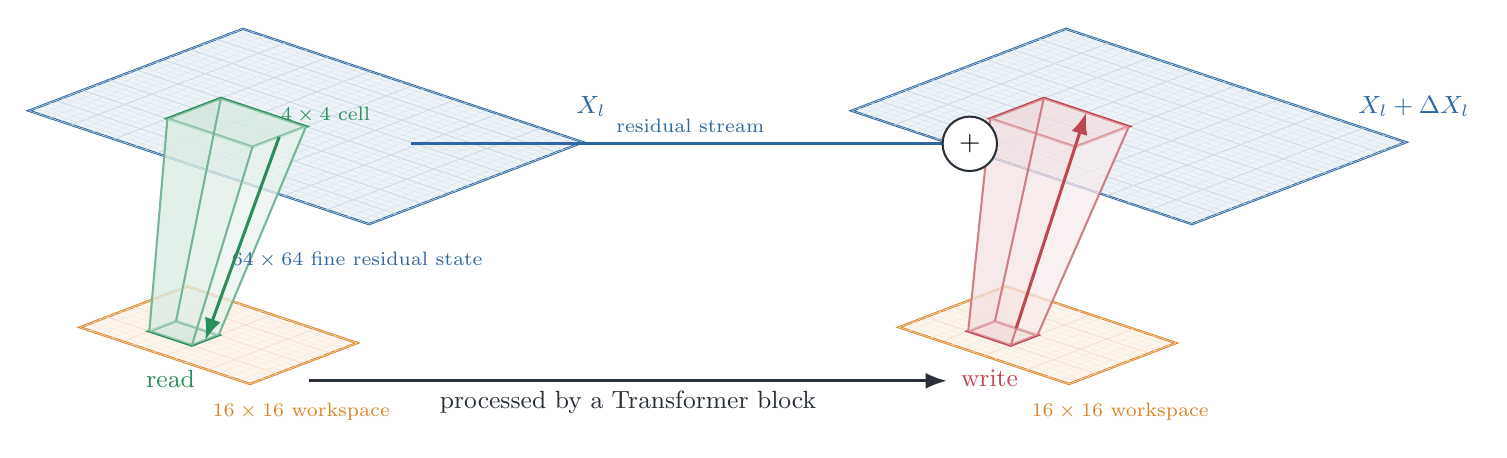
\begin{tikzpicture}[x=1cm,y=1cm]

  % Left read stack: high resolution -> workspace.
  \coordinate (readTop) at (-6.1,2.6);
  \coordinate (readBot) at (-5.45,-0.15);
  \gridplane{rt}{(readTop)}{8}{8}{fineblue}{1}
  \subgrid{(readTop)}{8}{8}{4}{fineblue}
  \gridplane{rb}{(readBot)}{4}{4}{workorange}{1}
  \subgrid{(readBot)}{4}{4}{4}{workorange}

  \cellpatch{rt}{(readTop)}{2}{2}{2}{2}{readgreen}{0.55}
  \cellpatch{rb}{(readBot)}{1}{1}{1}{1}{readgreen}{0.55}

  % Projection walls for read.
  \fill[readgreen!18, opacity=0.55]
    (rt-p0) -- (rt-p1) -- (rb-p1) -- (rb-p0) -- cycle;
  \fill[readgreen!12, opacity=0.50]
    (rt-p1) -- (rt-p2) -- (rb-p2) -- (rb-p1) -- cycle;
  \fill[readgreen!10, opacity=0.48]
    (rt-p2) -- (rt-p3) -- (rb-p3) -- (rb-p2) -- cycle;
  \fill[readgreen!16, opacity=0.52]
    (rt-p3) -- (rt-p0) -- (rb-p0) -- (rb-p3) -- cycle;
  \draw[readgreen!65, line width=0.75pt]
    (rt-p0) -- (rb-p0) (rt-p1) -- (rb-p1) (rt-p2) -- (rb-p2) (rt-p3) -- (rb-p3);

  \node[lab, text=fineblue] at ($(rt-c)+(0.1,0.45)$) {$X_l$};
  \node[tiny, text=fineblue] at ($(rt-b)+(-0.15,-0.45)$) {$64\times64$ fine residual state};
  \node[tiny, text=readgreen] at ($(rt-p2)+(0.25,0.15)$) {$4\times4$ cell};
  \node[lab, text=readgreen] at ($(rb-o)+(1.15,-0.65)$) {read};

  % Right write stack: workspace -> high resolution.
  \coordinate (writeTop) at (4.35,2.6);
  \coordinate (writeBot) at (4.95,-0.15);
  \gridplane{wt}{(writeTop)}{8}{8}{fineblue}{1}
  \subgrid{(writeTop)}{8}{8}{4}{fineblue}
  \gridplane{wb}{(writeBot)}{4}{4}{workorange}{1}
  \subgrid{(writeBot)}{4}{4}{4}{workorange}

  \cellpatch{wt}{(writeTop)}{2}{2}{2}{2}{writered}{0.45}
  \cellpatch{wb}{(writeBot)}{1}{1}{1}{1}{writered}{0.55}

  % Projection walls for write.
  \fill[writered!18, opacity=0.50]
    (wb-p0) -- (wb-p1) -- (wt-p1) -- (wt-p0) -- cycle;
  \fill[writered!12, opacity=0.48]
    (wb-p1) -- (wb-p2) -- (wt-p2) -- (wt-p1) -- cycle;
  \fill[writered!10, opacity=0.45]
    (wb-p2) -- (wb-p3) -- (wt-p3) -- (wt-p2) -- cycle;
  \fill[writered!16, opacity=0.50]
    (wb-p3) -- (wb-p0) -- (wt-p0) -- (wt-p3) -- cycle;
  \draw[writered!70, line width=0.75pt]
    (wb-p0) -- (wt-p0) (wb-p1) -- (wt-p1) (wb-p2) -- (wt-p2) (wb-p3) -- (wt-p3);

  \node[lab, text=fineblue] at ($(wt-c)+(0.1,0.45)$) {$X_l+\Delta X_l$};
  \node[lab, text=writered] at ($(wb-o)+(1.15,-0.65)$) {write};

  % Transformer processing on workspace level.
  \coordinate (rbCenter) at ($(rb-o)!0.5!(rb-c)$);
  \coordinate (wbCenter) at ($(wb-o)!0.5!(wb-c)$);
  \draw[flow] ($(rbCenter)+(1.15,-0.58)$) -- node[below, lab, text=ink]
    {processed by a Transformer block}
    ($(wbCenter)+(-1.15,-0.58)$);

  % Direction hints, kept straight and sparse.
  \draw[readflow] ($(rt-p3)!0.5!(rt-p2)$) -- ($(rb-p3)!0.5!(rb-p2)$);
  \draw[writeflow] ($(wb-p1)!0.5!(wb-p2)$) -- ($(wt-p1)!0.5!(wt-p2)$);

  \node[tiny, text=workorange] at ($(rb-b)+(0.65,-0.35)$) {$16\times16$ workspace};
  \node[tiny, text=workorange] at ($(wb-b)+(0.65,-0.35)$) {$16\times16$ workspace};

  % Residual stream on top, parallel to the workspace Transformer arrow.
  \coordinate (plus) at (5.85,2.18);
  \draw[residual] (-1.25,2.18) -- node[above, tiny, text=fineblue] {residual stream} (plus);
  \node[circle, draw=ink, fill=white, line width=0.75pt, minimum size=0.42cm] at (plus) {$+$};

\end{tikzpicture}
\end{document}
